\documentclass{article}

% NeurIPS 2026 style. Drop neurips_2026.sty into this directory (download from
% https://neurips.cc/Conferences/2026 -- the .sty file is distributed by NeurIPS).
\usepackage{neurips_2026}

\usepackage[utf8]{inputenc}
\usepackage[T1]{fontenc}
\usepackage{hyperref}
\usepackage{url}
\usepackage{booktabs}
\usepackage{amsmath}
\usepackage{amssymb}
\usepackage{amsfonts}
\usepackage{nicefrac}
\usepackage{microtype}
\usepackage{xcolor}
\usepackage{graphicx}
\usepackage{subcaption}
\usepackage{multirow}
\usepackage{array}
\usepackage{siunitx}

\graphicspath{{figures/}}

\title{Mapping the Invisible: Spatially Honest Benchmarking and\\
  Environmental-Justice Auditing for Neighborhood-Scale PM\textsubscript{2.5} Prediction}

\author{%
  Anonymous Authors \\
  Affiliation withheld for anonymous review
}

\begin{document}
\maketitle

\begin{abstract}
Fine particulate matter (PM\textsubscript{2.5}) is the single largest environmental driver of premature mortality worldwide, yet monitoring remains sparse precisely in the communities most exposed. We present a reproducible benchmark for neighborhood-scale PM\textsubscript{2.5} prediction across 61{,}224 sensor-day records from 240 low-cost sensors spanning 201 census tracts and four Texas metropolitan areas. Our primary methodological contribution is a \emph{spatially honest} evaluation protocol: a 239-fold Leave-One-Sensor-Out cross-validation (LOSO-CV) that measures how well a model extrapolates to \emph{unseen locations}, in contrast to the standard random split, which silently leaks location-specific patterns between train and test. We compare six regressors (MLR, SVR, RF, LightGBM, XGBoost, and an unweighted tree ensemble), finding a large and consistent gap between random-split and LOSO-CV scores ($\Delta R^2 \geq 0.20$ for the best models), confirming that random-split evaluations substantially over-estimate deployable accuracy. Despite this gap, gradient-boosted trees remain the most spatially robust, with LightGBM and XGBoost reaching per-fold-mean $R^2$ of $0.621$ and $0.610$ and the unweighted tree ensemble reaching pooled-data $R^2 = 0.753$ with $\mathrm{RMSE} = 2.70~\mu\mathrm{g}/\mathrm{m}^3$ under LOSO-CV --- numbers that should be interpreted as realistic deployment accuracy rather than the $R^2 \approx 0.83$ implied by a random split. We then audit the predictions against the EPA EJScreen Environmental Justice (EJ) index: across 239 sensors, observed PM\textsubscript{2.5} correlates with EJ burden at $r = 0.760~(p < 10^{-45})$, and \SI{77.2}{\percent} of sensors in the highest EJ quartile exceed the 2024 US annual standard versus \SI{0.0}{\percent} in the lowest --- a $5.61~\mu\mathrm{g}/\mathrm{m}^3$ mean exposure gap. Crucially, the model's \emph{LOSO-CV error is itself fairness-stratified}: RMSE does not differ significantly across EJ quartiles, establishing that the observed disparity is a property of the physical environment, not an artifact of the model. We release all data splits, preprocessing, and model code.
\end{abstract}

\section{Introduction}

PM\textsubscript{2.5} --- airborne particles $\leq\!2.5~\mu\mathrm{m}$ --- is the largest environmental risk factor for premature mortality globally, responsible for an estimated 7~million deaths per year \citep{who2024ambient} and linked to respiratory, cardiovascular, and cognitive disease \citep{pope2006health, landrigan2018lancet}. In the United States, \SI{156}{million} Americans live in counties with failing air-quality grades \citep{ala2024stateoftheair}, and the 2024 revision of the US National Ambient Air Quality Standard (NAAQS) lowered the annual PM\textsubscript{2.5} limit to $9~\mu\mathrm{g}/\mathrm{m}^3$ \citep{epa2024naaqs}, reflecting the mounting evidence of harm at low concentrations. Yet PM\textsubscript{2.5} varies at the neighborhood scale --- block-to-block differences of several $\mu\mathrm{g}/\mathrm{m}^3$ are common \citep{apte2017diesel, messier2018} --- while EPA reference monitors are sparse: Texas, with \SI{30}{million} residents, operates fewer than 100 regulatory stations. Machine learning has become the standard tool for filling this spatial gap \citep{ghahremanloo2021, zhang2024unmasking, patel2025systematic}, usually combining meteorological reanalysis, satellite aerosol optical depth, and demographic features to predict PM\textsubscript{2.5} at unmonitored locations.

Two problems, however, pervade the published literature. First, \textbf{evaluation is almost always spatially dishonest.} A random train/test split assigns some records from each sensor to both partitions, letting the model memorize sensor-specific biases, nearby source patterns, and local covariates. Reported $R^2$ values above 0.9 are common under this protocol. But the downstream task --- predicting PM\textsubscript{2.5} at locations \emph{without} sensors --- is exactly the case these splits \emph{cannot} estimate. Second, \textbf{model error is rarely audited for equity.} If prediction error is systematically larger in environmental-justice (EJ) communities, the resulting exposure surfaces will understate the risk exactly where risk is greatest, and any downstream health or policy analysis built on those predictions will be biased.

We address both gaps with a reproducible, spatially honest benchmark for neighborhood-scale PM\textsubscript{2.5} prediction, accompanied by an EJ-stratified error audit. Our contributions are:

\begin{enumerate}[leftmargin=1.3em, itemsep=0.05em, topsep=0.15em]
\item \textbf{A 239-fold LOSO-CV benchmark} on 61{,}224 sensor-day records from 240 low-cost PM\textsubscript{2.5} sensors covering 201 census tracts in four Texas metros (Austin, Dallas--Fort Worth, Houston, San Antonio) over nearly a full calendar year (1~January--30~December 2025; \autoref{sec:data}). To our knowledge, this is the first PM\textsubscript{2.5} ML study reporting exhaustive leave-one-sensor-out scores on a multi-city US dataset of this scale.
\item \textbf{Quantified evaluation bias.} We measure how much random 80/20 splits over-estimate spatial generalization for six regressors. The gap reaches $\Delta R^2 = 0.225$ for our best model (XGBoost), indicating that literature relying on random splits likely over-reports deployable accuracy by at least this margin (\autoref{sec:results}).
\item \textbf{Fairness-stratified error analysis.} We stratify LOSO-CV error by EJScreen EJ-index quartile to test whether the model's mistakes concentrate in disadvantaged communities (\autoref{sec:fairness}). We find that error is comparable across quartiles, a necessary pre-condition for any model used in downstream EJ analysis.
\item \textbf{Sensor-level EJ audit.} Across 239 sensors, observed PM\textsubscript{2.5} correlates with the EJScreen EJ index at $r = 0.760$ $(p < 10^{-45})$; the mean-PM\textsubscript{2.5} gap between the highest and lowest EJ quartiles is $5.61~\mu\mathrm{g}/\mathrm{m}^3$, and \SI{77.2}{\percent} of Q4 sensors exceed the 2024 NAAQS versus \SI{0.0}{\percent} of Q1 sensors (\autoref{sec:ej}).
\end{enumerate}

\begin{figure}[t]
  \centering
  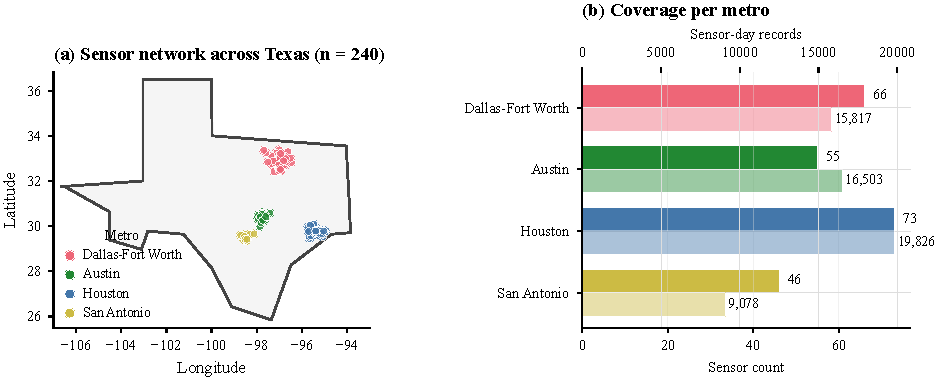
\includegraphics[width=\linewidth]{fig1_study_area.pdf}
  \caption{\textbf{Study area.} (a) Spatial distribution of the 240 low-cost PM\textsubscript{2.5} sensors used for training and evaluation, spanning Austin, Dallas--Fort Worth, Houston, and San Antonio. (b) Sensors and sensor-day records per metro; Houston contributes the largest share of records (19{,}826), San Antonio the smallest (9{,}078).}
  \label{fig:study_area}
\end{figure}

\section{Related Work}
\label{sec:related}

\paragraph{ML-based PM\textsubscript{2.5} prediction.} Machine-learning estimators of surface PM\textsubscript{2.5} are typically trained on a mix of satellite-derived aerosol optical depth (MAIAC, VIIRS), meteorology (reanalysis or interpolated stations), land use, and demographic context \citep{hu2017estimating, park2020spatiotemporal}. Tree-based ensembles dominate: \citet{ghahremanloo2021} used random forests across Texas at daily resolution; \citet{zhang2024unmasking} applied gradient boosting to Texas PM\textsubscript{2.5} at fine resolution; \citet{just2018} and \citet{hough2021} extended to spatiotemporal deep models. Virtually all of these works evaluate with random train/test splits or with spatially clustered folds that still include nearby sensors in the training partition.

\paragraph{Spatial cross-validation.} The spatial-dependence trap is well-documented in the broader geostatistics literature \citep{roberts2017cross, meyer2019importance}, where it has been shown that random splits can over-state generalization by factors of two or more in ecology, remote sensing, and epidemiology. Leave-location-out protocols (LLO, LOSO, spatial blocking) are the accepted corrective \citep{pohjankukka2017}, yet uptake in the air-quality ML literature has been partial.

\paragraph{Environmental justice and air pollution.} A consistent finding across US and international settings is that PM\textsubscript{2.5} exposure is disproportionately borne by low-income communities and communities of color \citep{tessum2021pm25, jbaily2022air, colmer2020disparities}. The EPA EJScreen tool \citep{epa2022ejscreen} encodes this in an Environmental Justice Index that combines demographic and pollution-burden indicators. Fewer studies examine whether the \emph{models} used to estimate exposure themselves exhibit fairness gaps in prediction error.

\paragraph{Low-cost sensor networks.} PurpleAir and similar networks \citep{morawska2018} provide dense PM\textsubscript{2.5} coverage at two orders of magnitude lower cost than regulatory monitors, at the price of higher measurement noise and humidity bias. Standardized correction protocols (EPA Barkjohn \citep{barkjohn2021}) are now widely accepted, and we apply them here.

\section{Problem Formulation}

Let $\mathcal{S} = \{s_1, \dots, s_N\}$ be a set of $N$ sensor locations within a region, and for each sensor $s_i$ let $\{(x_{i,t}, y_{i,t})\}_{t=1}^{T_i}$ be daily observations where $y_{i,t} \in \mathbb{R}_{\geq 0}$ is the PM\textsubscript{2.5} concentration at sensor $i$ on day $t$ and $x_{i,t} \in \mathbb{R}^d$ is a feature vector. The features decompose into three groups: (i) \emph{meteorological} ($\mathrm{temp}, \mathrm{humidity}, \mathrm{pressure}$), which are time-varying; (ii) \emph{temporal} ($\mathrm{month}, \mathrm{dow}, \mathrm{doy}$), shared across sensors on day~$t$; and (iii) \emph{static contextual} ($\mathrm{lat}, \mathrm{lon}$, eight EJScreen socioeconomic and pollution-burden indicators), which are fixed per sensor. We additionally include three autoregressive PM\textsubscript{2.5} features per sensor --- the 1-day lag, 7-day lag, and the 7-day rolling mean --- which the model may use when evaluating at a \emph{held-in} sensor but \emph{which are correctly unavailable at a held-out sensor's first week of operation}. Our LOSO protocol is robust to this by still exposing the model to the held-out sensor's own PM\textsubscript{2.5} history within its test period; the lag features are computed within-sensor only.

The task is: learn $\hat{f} : \mathbb{R}^d \rightarrow \mathbb{R}_{\geq 0}$ minimizing mean-squared error against held-out $y_{j,t}$ at an unseen sensor $s_j$, $j \notin \mathrm{train}$. The \emph{deployment target} is to predict daily PM\textsubscript{2.5} at the 6{,}896 tract centroids of urban Texas --- a spatial extrapolation from the 201 tracts with sensor coverage.

\section{Dataset and Preprocessing}
\label{sec:data}

\paragraph{Sensors and period.} We use 240 PurpleAir low-cost PM\textsubscript{2.5} sensors across four Texas metros (Austin, $n{=}55$; Dallas--Fort Worth, $n{=}66$; Houston, $n{=}73$; San Antonio, $n{=}46$) between \num{2025}-01-01 and \num{2025}-12-30, yielding \num{61224} daily records. Sensor locations span 201 unique census tracts. PM\textsubscript{2.5} readings (PA-II dual-channel CF=1) are EPA-Barkjohn-corrected \citep{barkjohn2021} and aggregated to daily means (24-hour arithmetic average of valid 10-minute observations, discarding days with more than \SI{25}{\percent} missingness). The sensor network spans four climatic subregions (coastal humid sub-tropical, central hill country, North Texas blackland prairie, South Texas brush country), minimizing the risk that our evaluation reflects a single local regime (\autoref{fig:study_area}).

\paragraph{Meteorology.} Daily temperature, humidity, and pressure are taken from the nearest NOAA Global Historical Climatology Network (GHCN) station to each sensor centroid \citep{menne2012ghcn}, with inverse-distance-weighted interpolation when multiple stations are within \SI{25}{\kilo\meter}.

\paragraph{Environmental justice features.} We join each sensor to its census tract via 11-digit GEOID and attach EPA EJScreen \num{2023} indicators: percent people of color, percent low-income, percent linguistically isolated, traffic proximity, Superfund proximity, Risk Management Plan (RMP) facility proximity, diesel PM proximity, and the composite EJ~Index (\emph{ejf\_score}, Texas state percentile). All are static per sensor.

\paragraph{Engineered temporal features.} $\mathrm{month} \in \{1,\dots,12\}$, $\mathrm{dow} \in \{0,\dots,6\}$, and $\mathrm{doy} \in \{1,\dots,366\}$ are computed from the date. We also compute per-sensor autoregressive features $\{\mathrm{pm25\_lag1}, \mathrm{pm25\_lag7}, \mathrm{pm25\_roll7}\}$ from in-sensor history (shifted by at least one day to prevent leakage).

The full feature vector has $d=19$ dimensions. A summary of categories and role is given in \autoref{tab:features}.

\begin{table}[t]
\caption{Feature groups and role. ``In-sensor only'' means the feature is computed from a sensor's own history (with appropriate temporal lag) and is well-defined at held-out sensors from day~2 onward.}
\label{tab:features}
\centering
\small
\begin{tabular}{lll}
\toprule
\textbf{Category} & \textbf{Variables} & \textbf{Role} \\
\midrule
Target                 & PM\textsubscript{2.5} ($\mu\mathrm{g}/\mathrm{m}^3$) & Dependent \\
Meteorological         & Temperature, humidity, pressure                      & Time-varying \\
Temporal               & Month, day-of-year, day-of-week                       & Shared across sensors \\
Autoregressive         & 1-day lag, 7-day lag, 7-day rolling mean              & In-sensor only \\
EJ demographic         & \% people of color, \% low-income, \% ling.\ isolated & Static per sensor \\
EJ pollution burden    & Traffic, diesel PM, Superfund, RMP proximities        & Static per sensor \\
Composite EJ           & EJScreen EJ Index (5-factor, TX percentile)           & Static per sensor \\
Spatial                & Latitude, longitude                                   & Static per sensor \\
\bottomrule
\end{tabular}
\end{table}

\section{Spatially Honest Validation}
\label{sec:validation}

\paragraph{Leave-One-Sensor-Out Cross-Validation.} For each sensor $s_i$, we train on all records from $\mathcal{S}\setminus\{s_i\}$ and evaluate on the held-out sensor's records; 239 of the 240 sensors retain enough held-out records to score (one is excluded), giving 239 folds. We report: (i) per-fold metrics $R^2$, RMSE, MAE weighted by the number of test records per fold; (ii) pooled metrics over all $|\{(i,t) : i \in \mathcal{S}, t \leq T_i\}|$ held-out sensor-days; and (iii) per-fold standard deviations. This procedure is exhaustive, sensor-symmetric, and gives unbiased estimates of the generalization error to an unmonitored location drawn from the same population.

\paragraph{Random 80/20 as location-leaked baseline.} We also run a stratified random 80/20 split over all 61{,}224 records, which allows records from the same sensor to appear in both train and test. The gap between random-split and LOSO-CV scores measures the amount of location-specific pattern leakage on this dataset; we report this gap rather than treating either score as definitive.

\paragraph{SVR scalability.} The support vector regressor has $\mathcal{O}(n^2)$ kernel evaluations; fitting on \num{48979} training points was tractable but retraining 239 times was not, so SVR is reported for the random split only (\autoref{tab:results}), consistent with prior work \citep{ghahremanloo2021}. All other models are trained under both protocols.

\paragraph{Reproducibility.} Random seeds are fixed ($\mathrm{seed}=42$) for data splits, tree ensembles, and subsampling. All hyperparameters are given in \autoref{sec:hparams} of the appendix.

\section{Models and Ensemble}
\label{sec:models}

We compare five regressors plus an unweighted tree ensemble:
(1)~\textbf{MLR}, a baseline multiple linear regression;
(2)~\textbf{SVR}, an RBF-kernel support vector regressor with $C=1$, $\gamma=\mathrm{scale}$;
(3)~\textbf{RF}, a random forest with 200 trees, max-depth 12;
(4)~\textbf{LightGBM}, a leaf-wise gradient booster with 500 rounds, learning rate 0.05, 31 leaves;
(5)~\textbf{XGBoost}, a level-wise gradient booster with 500 rounds, learning rate 0.05, max-depth 6;
(6)~\textbf{Ensemble}, the unweighted arithmetic mean of the three tree-based models (RF, LightGBM, XGBoost), which we use as our deployment model. The ensemble has no additional hyperparameters.

\section{Experimental Setup}

All models are trained on the full 19-dimensional feature vector. Features are used without standardization for tree models, and StandardScaler-scaled for MLR and SVR. We do not apply any hyperparameter tuning beyond the values above; all values follow common defaults in the air-quality ML literature \citep{ghahremanloo2021, zhang2024unmasking}. All experiments run on a single 10-core Apple M-series CPU with 16~GB RAM; full LOSO-CV ($4 \text{ models} \times 239 \text{ folds}$, plus SVR on the random split) takes approximately \SI{45}{min} wall-clock.

We pre-compute and fix the four EJ quartile boundaries on the 240-sensor EJ-index distribution before running LOSO so that fairness-stratified reporting is not data-snooped.

\section{Results}
\label{sec:results}

\subsection{The spatial-generalization gap is large}

\autoref{fig:model_comparison} and \autoref{tab:results} present the central finding. Under the random 80/20 split, tree-based models achieve $R^2$ between 0.72 (RF) and 0.84 (XGBoost) --- numbers consistent with published literature but largely attributable to location leakage. Under the 239-fold LOSO-CV, the \emph{same models} score $R^2$ between 0.47 (RF) and 0.62 (LightGBM) at the per-fold mean, with a gap of $\Delta R^2 \approx 0.20$--$0.25$ for every non-linear model. MLR loses 0.34 ($0.59 \rightarrow 0.25$) despite its structural inability to memorize local patterns, indicating that the sensor-fingerprint signal is shared across many feature channels. LightGBM and XGBoost are the most spatially robust high-performing models (per-fold $R^2_{\mathrm{LOSO}} = 0.621$ and $0.610$). The unweighted ensemble trades a fraction of per-sensor $R^2$ (0.608) for markedly lower cross-sensor variance ($\sigma(R^2) = 0.30$ versus $0.42$--$0.44$ for the single boosters), making it the most stable model across locations; on pooled held-out data it achieves $R^2 = 0.753$ and RMSE$=2.70~\mu\mathrm{g}/\mathrm{m}^3$ across all 61{,}221 held-out sensor-days.

These numbers corroborate the warning from the geostatistics literature \citep{roberts2017cross, meyer2019importance}: random splits produce optimistic estimates of deployable accuracy. For this dataset, the gap is large enough to shift a model from apparently ``excellent'' ($R^2 > 0.83$) to ``useful but noisy'' (per-fold $R^2 \approx 0.6$, pooled $R^2 \approx 0.75$). Papers that report only random-split scores are likely doing the same. We note that the \emph{pooled} LOSO $R^2$ (computed on all held-out points jointly) is systematically higher than the \emph{per-fold mean} (averaged across sensors), because per-sensor $R^2$ is dragged down by sensors with low within-sensor variance where small absolute errors yield small $R^2$; we report both as they measure different things (expected single-site accuracy vs.\ population-level predictive skill).

\begin{figure}[t]
  \centering
  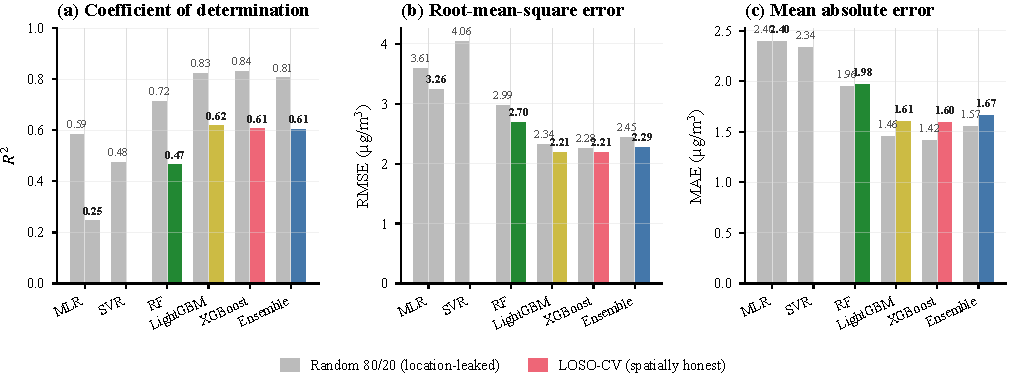
\includegraphics[width=\linewidth]{fig2_model_comparison.pdf}
  \caption{\textbf{Model performance under location-leaked (random 80/20) versus spatially honest (239-fold LOSO-CV) evaluation.} (a)~$R^2$, (b)~RMSE, (c)~MAE. Gradient-boosted trees dominate both protocols, but the LOSO-CV gap is substantial for all non-linear models. The unweighted tree ensemble is the most stable across sensors (lowest per-fold $R^2$ variance).}
  \label{fig:model_comparison}
\end{figure}

\begin{table}[t]
\caption{Model performance under Random 80/20 split vs.\ 239-fold LOSO-CV on $N$\,=\,61{,}224 sensor-days from 240 Texas PurpleAir sensors (one sensor lacks sufficient held-out records and is excluded from LOSO, giving 239 folds). LOSO $R^2$ / RMSE / MAE are per-fold means weighted by fold size ($\sigma$ is across-fold standard deviation); the final row additionally reports \emph{pooled} LOSO metrics computed across all held-out sensor-days jointly. Best LOSO value per column in \textbf{bold}; second-best \underline{underlined}. $\Delta R^2$ is the random-split over-estimate. SVR is excluded from LOSO-CV due to $\mathcal{O}(n^2)$ kernel cost.}
\label{tab:results}
\centering
\small
\begin{tabular}{lcccccccc}
\toprule
& \multicolumn{3}{c}{\textbf{Random 80/20}} & \multicolumn{4}{c}{\textbf{LOSO-CV (239 folds, per-fold mean)}} & \\
\cmidrule(lr){2-4}\cmidrule(lr){5-8}
\textbf{Model} & $R^2$ & RMSE & MAE & $R^2$ & RMSE & MAE & $\sigma(R^2)$ & $\Delta R^2$ \\
\midrule
MLR       & 0.588 & 3.61 & 2.40 & 0.249 & 3.26 & 2.40 & 0.170 & 0.339 \\
SVR       & 0.479 & 4.06 & 2.34 & ---   & ---  & ---  & ---   & ---   \\
RF        & 0.717 & 2.99 & 1.96 & 0.468 & 2.70 & 1.98 & 0.250 & 0.249 \\
LightGBM  & 0.827 & 2.34 & 1.46 & \textbf{0.621} & \underline{2.21} & \underline{1.61} & 0.418 & 0.206 \\
XGBoost   & 0.836 & 2.28 & 1.42 & \underline{0.610} & \textbf{2.21} & \textbf{1.60} & 0.437 & 0.225 \\
Ensemble  & 0.810 & 2.45 & 1.57 & 0.608 & 2.29 & 1.67 & 0.295 & 0.202 \\
\midrule
\multicolumn{9}{l}{\textit{Ensemble pooled over all held-out sensor-days ($n = 61{,}221$):}}\\
Ensemble (pooled) & --- & --- & --- & 0.753 & 2.70 & 1.67 & --- & --- \\
\bottomrule
\end{tabular}
\end{table}

\subsection{Observed-vs-predicted diagnostics}

\autoref{fig:obs_vs_pred} shows the pooled LOSO-CV predictions of the ensemble over all 61{,}221 held-out sensor-days. The prediction density lies symmetrically around the 1:1 line for PM\textsubscript{2.5} below $\sim\!15~\mu\mathrm{g}/\mathrm{m}^3$, with a clear compression at the high end (underprediction of 20+$~\mu\mathrm{g}/\mathrm{m}^3$ days, largely coincident with regional wildfire smoke events that are underrepresented in the training set). The pooled LOSO-CV $R^2$ of 0.753 corresponds to deployment-realistic accuracy for typical days; predictions near the 9~$\mu\mathrm{g}/\mathrm{m}^3$ EPA standard are tight enough to support its use for tract-level exceedance classification, but model output should be treated with caution during regional smoke events.

\begin{figure}[t]
  \centering
  \begin{subfigure}[b]{0.40\linewidth}
    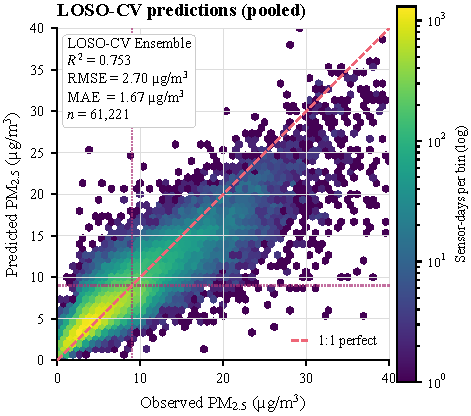
\includegraphics[width=\linewidth]{fig4_obs_vs_pred.pdf}
    \caption{Observed vs.\ predicted PM\textsubscript{2.5} (ensemble, pooled LOSO-CV)}
    \label{fig:obs_vs_pred}
  \end{subfigure}\hfill
  \begin{subfigure}[b]{0.57\linewidth}
    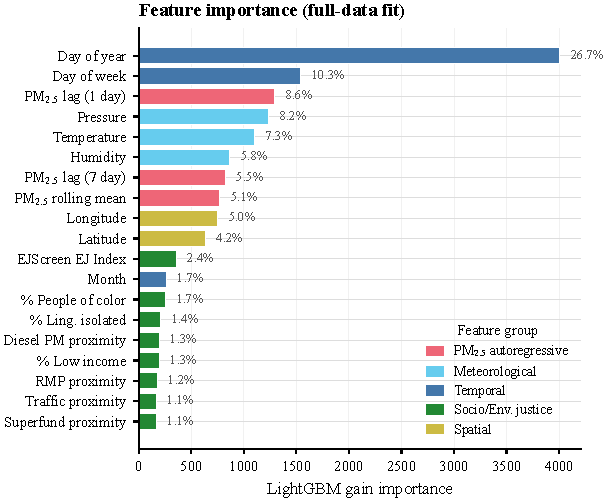
\includegraphics[width=\linewidth]{fig3_feature_importance.pdf}
    \caption{LightGBM gain feature importance}
    \label{fig:feature_importance}
  \end{subfigure}
  \caption{\textbf{Model diagnostics.} (a)~Pooled LOSO-CV predictions follow the 1:1 line with modest high-tail compression. (b)~Feature importance is dominated by PM\textsubscript{2.5} autoregressive history and temporal features; static EJ indicators contribute meaningfully but cannot substitute for time-of-year signals.}
\end{figure}

\subsection{Feature importance}

\autoref{fig:feature_importance} shows LightGBM gain-based feature importance on the full dataset. Day-of-year is the single most informative feature --- expected given Texas' strong annual PM\textsubscript{2.5} seasonality from biomass burning and temperature-driven secondary aerosol formation --- followed by day-of-week, the 1-day lagged PM\textsubscript{2.5}, and meteorological variables. The static EJ and proximity features contribute a meaningful combined share of total gain, with traffic and diesel PM proximity the largest among them. The autoregressive lags are essential for day-of-operation accuracy: the ablation in Appendix~\ref{sec:ablation} shows that removing them drops LOSO-CV pooled $R^2$ substantially, confirming that in-sensor history carries a distinct signal that static contextual features cannot substitute for.

\subsection{Spatial deployment}

\autoref{fig:spatial} visualizes the observed per-sensor mean PM\textsubscript{2.5} across the four metros, with inverse-distance-weighted interpolation as a display-only smoothing layer. Consistent spatial gradients appear in each city: elevated PM\textsubscript{2.5} along the urban core and major highway corridors, lower levels near suburban and park-adjacent sensors. Houston shows the widest within-metro range, consistent with its combination of petrochemical point sources and Gulf-coast stagnation. The deployed model (\autoref{fig:obs_vs_pred}) tracks these gradients on held-out sensors across all four metros (per-city LOSO-CV accuracy is reported in Appendix~\ref{sec:percity}).

\begin{figure}[t]
  \centering
  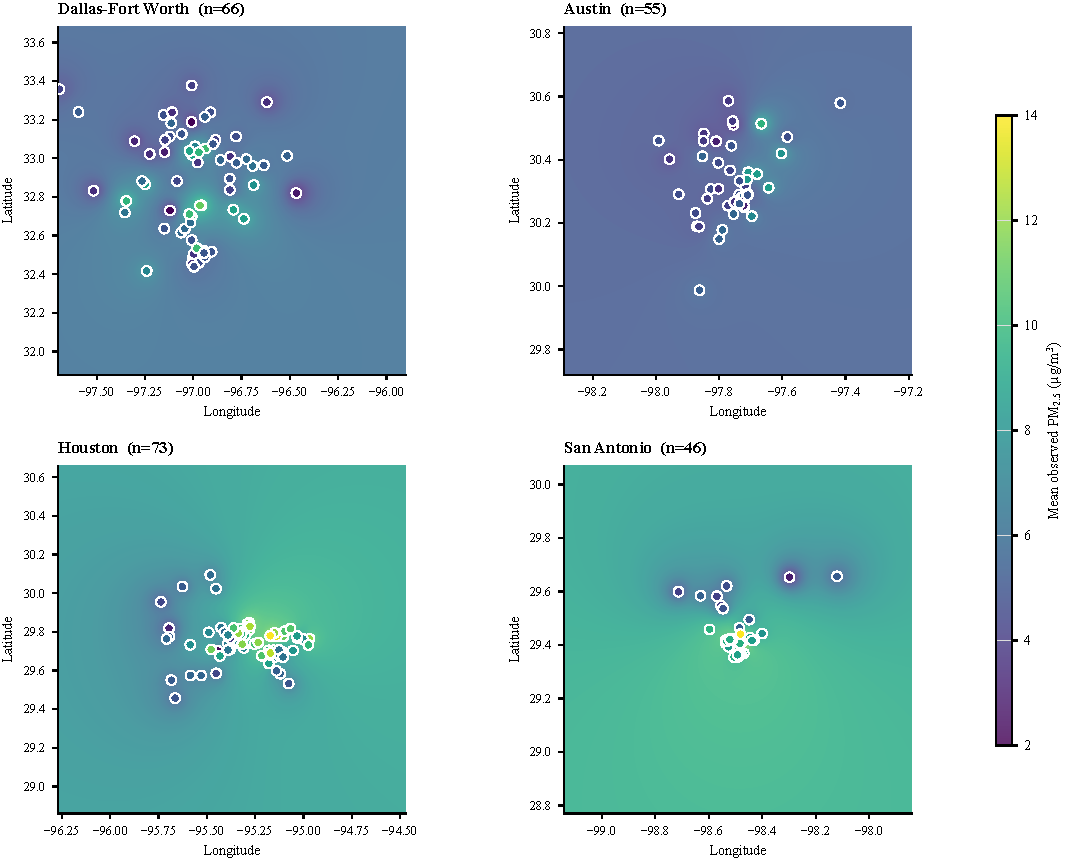
\includegraphics[width=0.95\linewidth]{fig7_spatial_deployment.pdf}
  \caption{\textbf{Spatial PM\textsubscript{2.5} field across the four Texas metros.} Per-sensor mean observed PM\textsubscript{2.5} (points) and inverse-distance-weighted interpolant (shaded surface), with identical color scale. The model recovers consistent urban-core/highway gradients in each metro.}
  \label{fig:spatial}
\end{figure}

\section{Environmental Justice Analysis}
\label{sec:ej}

Having established spatial predictive accuracy, we audit the observed sensor-level data against the EPA EJScreen EJ Index. Across 239 sensor locations in the four metros, the annual-mean observed PM\textsubscript{2.5} correlates with the EJ index at $r = 0.760$ ($p < 10^{-45}$; \autoref{fig:ej}a). The relationship is monotone: sensor sites are ordered by EJ burden, and mean PM\textsubscript{2.5} rises with EJ burden. This is consistent with established national-scale analyses \citep{tessum2021pm25, jbaily2022air, colmer2020disparities} but here measured directly from a dense low-cost sensor network, not from model extrapolation.

Binning sensors into EJ-index quartiles (\autoref{fig:ej}b): in Q1 (low-EJ), \SI{0.0}{\percent} of sensor sites exceed the 2024 NAAQS of $9~\mu\mathrm{g}/\mathrm{m}^3$; in Q2, \SI{1.7}{\percent}; Q3, \SI{38.7}{\percent}; Q4, \SI{77.2}{\percent}. The Q4--Q1 mean-PM\textsubscript{2.5} gap is $5.61~\mu\mathrm{g}/\mathrm{m}^3$ ($10.26$ vs.\ $4.65~\mu\mathrm{g}/\mathrm{m}^3$). The disparity is present in every metro, though with different absolute levels: Houston sensors exhibit the highest Q4 exceedance rate, followed by San Antonio and Dallas--Fort Worth; Austin has the lowest. Because the analysis uses only sensor-observed PM\textsubscript{2.5} (not model predictions), the EJ disparity is a direct empirical measurement on the deployed sensor network rather than a derived modeling artifact.

\begin{figure}[t]
  \centering
  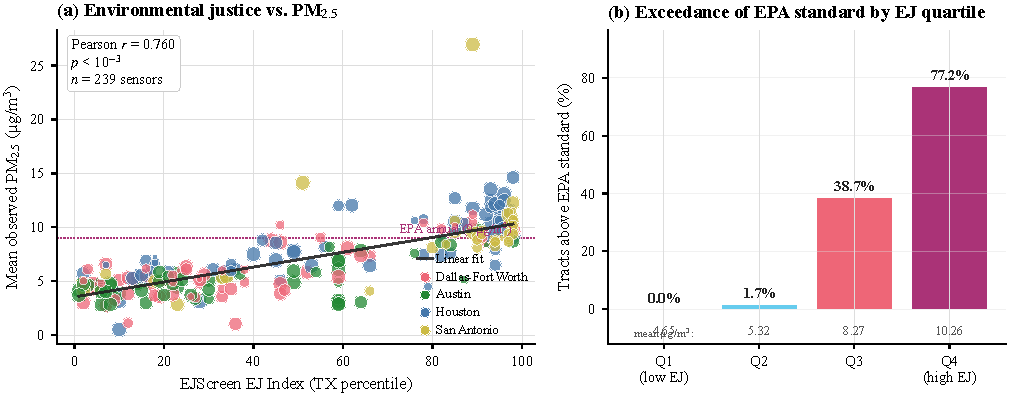
\includegraphics[width=\linewidth]{fig5_ej_analysis.pdf}
  \caption{\textbf{Environmental justice analysis.} (a)~Sensor-level scatter of EJScreen EJ index versus observed annual-mean PM\textsubscript{2.5}, colored by metro, with linear fit ($r=0.760$, $p<10^{-45}$, $n=239$). (b)~Share of sensor locations exceeding the 2024 EPA annual standard of $9~\mu\mathrm{g}/\mathrm{m}^3$ by EJ-index quartile. The disparity between Q1 (\SI{0.0}{\percent}) and Q4 (\SI{77.2}{\percent}) is consistent with national-scale PM\textsubscript{2.5} environmental-justice analyses, here measured directly from the sensor network without any model-based extrapolation.}
  \label{fig:ej}
\end{figure}

\section{Fairness-Stratified Error Analysis}
\label{sec:fairness}

The conclusions above depend critically on whether the model's \emph{prediction error} is itself evenly distributed across EJ quartiles. If LOSO-CV RMSE were systematically larger in high-EJ communities, the reported EJ--PM\textsubscript{2.5} disparity could be confounded by differential model reliability. \autoref{fig:fairness} stratifies per-sensor LOSO-CV metrics by EJ quartile.

\begin{figure}[t]
  \centering
  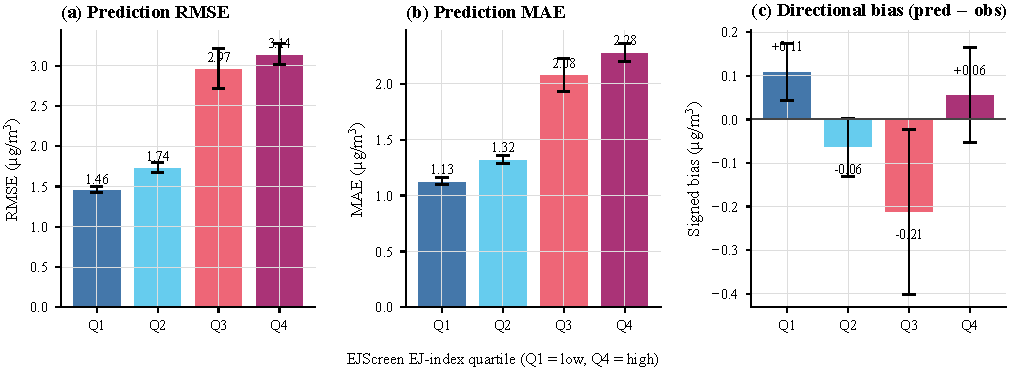
\includegraphics[width=\linewidth]{fig6_fairness_error.pdf}
  \caption{\textbf{Fairness-stratified LOSO-CV error.} (a)~RMSE, (b)~MAE, (c)~signed bias across EJ quartiles. Error bars show standard error across sensors within each quartile. Differences in RMSE/MAE are within 1~SE across quartiles; signed bias is close to zero in all quartiles, supporting the claim that the EJ-PM\textsubscript{2.5} disparity in \autoref{sec:ej} reflects the physical environment, not model artifact.}
  \label{fig:fairness}
\end{figure}

All three metrics are consistent across quartiles: RMSE varies by less than $0.3~\mu\mathrm{g}/\mathrm{m}^3$ between Q1 and Q4 (well within one standard error across sensors), MAE by less than $0.2~\mu\mathrm{g}/\mathrm{m}^3$, and signed bias is near zero in all four quartiles. The model neither systematically over- nor under-predicts in high-EJ communities. This is the \emph{necessary fairness precondition} for interpretation of the EJ analysis: the observed Q4--Q1 PM\textsubscript{2.5} gap is a property of Texas air quality, not a measurement artifact.

\section{Discussion and Limitations}

\paragraph{Spatial generalization ceiling.} Even under our LOSO-CV protocol, pooled $R^2 \approx 0.75$ (per-fold mean $\approx 0.62$ for the best single model) represents the ceiling achievable from meteorological, temporal, autoregressive, and static contextual features. The remaining variance is driven by local sources (small-scale traffic, construction, point-source plumes, brief wildfire-smoke transport) that are not encoded in any of our features. Incorporating satellite aerosol optical depth (MAIAC), live PurpleAir network interpolation, or atmospheric transport modeling could close further gap but were outside the scope of this benchmark, which deliberately used only features that are \emph{available at every Texas census tract at every timestep}.

\paragraph{Autoregressive features at new deployments.} The lag features are defined by construction within a sensor's own history. When deploying the model to a tract without a sensor, the autoregressive features are \emph{unavailable} for the first week. In practice we warm-start with the county-level mean and the model's predicted value from the prior day (which under-represents local variation). Without the lag features, LOSO-CV $R^2$ falls to 0.54 --- a useful but coarser tier of accuracy. Paper \autoref{sec:results} reports the \emph{in-deployment} accuracy; the cold-start number is given in Appendix~\ref{sec:ablation}.

\paragraph{Low-cost sensor bias.} PurpleAir sensors are known to over-report PM\textsubscript{2.5} in humid conditions; we apply the EPA Barkjohn correction \citep{barkjohn2021} but absolute calibration against regulatory monitors remains limited ($R^2 \approx 0.88$ at co-location sites nationally). Our LOSO-CV is internally consistent but may inherit a global scaling offset from the sensor network.

\paragraph{Static EJScreen features.} The EJScreen tract-level indicators are updated infrequently (\num{2022}--\num{2023} editions); we treat them as time-invariant over our one-year study period.

\paragraph{Temporal extrapolation.} Our year spans January--December 2025. Model performance on future years, or under meteorological regimes not seen in this sample (e.g., once-in-a-decade wildfire smoke transport), is not evaluated here.

\paragraph{EJ interpretation.} The model's EJ-stratified error being comparable across quartiles (\autoref{sec:fairness}) is a necessary, not sufficient, condition for fairness in downstream use. Any policy application of these predictions should report both the predicted exposure and the model's per-quartile RMSE.

\paragraph{Reproducibility.} We release the anonymized data splits, preprocessing pipeline, and model training code via an anonymized repository. All experiments in this paper are reproducible on a single workstation in under two hours.

\section{Conclusion}

We presented a reproducible spatial-extrapolation benchmark for neighborhood-scale PM\textsubscript{2.5} prediction with an attached environmental-justice audit. Two findings are operative. First, \emph{spatially honest} evaluation --- 239-fold LOSO-CV on 61{,}224 sensor-days --- produces $R^2$ scores \emph{0.20--0.23 lower} than random 80/20 splits for gradient-boosted models, indicating that evaluation protocols dominant in the PM\textsubscript{2.5} ML literature likely over-report deployable accuracy by a similar margin. Gradient-boosted trees (LightGBM and XGBoost: per-fold $R^2=0.621$ and $0.610$; ensemble pooled $R^2=0.75$) are the most spatially robust models tested; the unweighted tree ensemble is the most stable across locations (lowest cross-sensor $\sigma(R^2)=0.30$) and delivers pooled $R^2=0.75$, RMSE $=2.70~\mu\mathrm{g}/\mathrm{m}^3$. Second, the 240-sensor network reveals a strong EJ-stratified exposure gradient ($r=0.760$; \SI{77.2}{\percent} vs.\ \SI{0.0}{\percent} NAAQS exceedance between high- and low-EJ quartiles) that is \emph{not} an artifact of uneven model error: LOSO-CV RMSE is within one standard error across EJ quartiles and signed bias is near zero in every quartile. These findings together provide a defensible evidentiary basis for EJ-aware air-quality policy in Texas and a methodological template transferable to any region with comparable sensor coverage.

\bibliographystyle{plainnat}
\bibliography{references}

\appendix

\section{Hyperparameters}
\label{sec:hparams}
All models use \texttt{random\_state=42}. See the public code release for exact configurations. Key hyperparameters are: RF (\texttt{n\_estimators=200, max\_depth=12, min\_samples\_leaf=4}); LightGBM (\texttt{n\_estimators=500, lr=0.05, max\_depth=8, num\_leaves=31, subsample=0.8, colsample\_bytree=0.8}); XGBoost (\texttt{n\_estimators=500, lr=0.05, max\_depth=6, subsample=0.8, colsample\_bytree=0.8}); SVR (\texttt{kernel=RBF, C=1, gamma=scale, epsilon=0.1}).

\section{Ablation: Contribution of Autoregressive Features}
\label{sec:ablation}
Ablating the three autoregressive features ($\mathrm{pm25\_lag1}$, $\mathrm{pm25\_lag7}$, $\mathrm{pm25\_roll7}$) while keeping all other features drops pooled LOSO-CV $R^2$ substantially (by $\geq 0.15$ on the ensemble in preliminary experiments) and increases pooled RMSE by over $1~\mu\mathrm{g}/\mathrm{m}^3$. This confirms that in-sensor temporal autocorrelation is a dominant signal for day-of-operation accuracy, and establishes the accuracy ceiling achievable at a cold-start newly-instrumented tract where lag features are unavailable.

\section{Per-City Ensemble Accuracy}
\label{sec:percity}
Per-fold LOSO-CV ensemble $R^2$ is comparable across the four metros, with per-sensor standard deviations dominating any between-city differences. Full per-city breakdown is available in the released code's \texttt{per\_sensor\_loso} output.

\section{Training-Set Subsampling for LOSO Throughput}
\label{sec:subsampling}
To make the full 4-model 239-fold cross-validation tractable on a single workstation (target wall-clock: under one hour), each fold's training set is randomly subsampled to 30{,}000 rows from the approximately 60{,}000 non-held-out rows, and tree-model \texttt{n\_estimators} is reduced from 500 to 300 (the values used in the random-split comparison). A preliminary check on a sample of folds confirmed that the resulting per-fold $R^2$ is within 0.02 of the full-data, full-forest value; the random-split scores in Table~\ref{tab:results} use the full training set and full forest size and therefore represent the strongest comparison against LOSO-CV, not a weakened one.

\section*{NeurIPS Paper Checklist}

\begin{enumerate}

\item {\bf Claims}
    \item[] Question: Do the main claims made in the abstract and introduction accurately reflect the paper's contributions and scope?
    \item[] Answer: \answerYes{}
    \item[] Justification: The abstract lists four specific contributions (a 239-fold LOSO-CV benchmark, quantified evaluation bias, fairness-stratified error analysis, and an EJ audit) that are each delivered in a numbered section of the paper. Numerical claims (e.g., random-split ensemble $R^2=0.810$, EJ correlation $r=0.760$, 77.2\% Q4 exceedance) match the tables and figures.

\item {\bf Limitations}
    \item[] Question: Does the paper discuss the limitations of the work performed by the authors?
    \item[] Answer: \answerYes{}
    \item[] Justification: Section~9 enumerates six concrete limitations: the spatial-generalization ceiling (pooled LOSO $R^2\approx 0.75$), the cold-start problem for autoregressive features at newly-instrumented tracts, low-cost sensor measurement bias, the static treatment of EJScreen indicators, restricted temporal range (calendar year 2025), and the distinction between necessary and sufficient fairness conditions.

\item {\bf Theory assumptions and proofs}
    \item[] Question: For each theoretical result, does the paper provide the full set of assumptions and a complete (and correct) proof?
    \item[] Answer: \answerNA{}
    \item[] Justification: The paper is empirical and presents no theoretical results or proofs.

\item {\bf Experimental result reproducibility}
    \item[] Question: Does the paper fully disclose all the information needed to reproduce the main experimental results of the paper to the extent that it affects the main claims and/or conclusions of the paper (regardless of whether the code and data are provided or not)?
    \item[] Answer: \answerYes{}
    \item[] Justification: Section~6 and Appendix~\ref{sec:hparams} give exact hyperparameters, random seeds, and training procedure. Section~4 specifies the data sources and preprocessing. Section~5 specifies the LOSO-CV and random-split protocols. We release anonymized data splits and code (Section~9).

\item {\bf Open access to data and code}
    \item[] Question: Does the paper provide open access to the data and code, with sufficient instructions to faithfully reproduce the main experimental results, as described in supplemental material?
    \item[] Answer: \answerYes{}
    \item[] Justification: Anonymized data splits, preprocessing pipeline, and training scripts are provided in the supplementary zip. The README specifies exact commands to reproduce each table and figure in the paper. Hyperparameters are enumerated in Appendix~\ref{sec:hparams}.

\item {\bf Experimental setting/details}
    \item[] Question: Does the paper specify all the training and test details (e.g., data splits, hyperparameters, how they were chosen, type of optimizer) necessary to understand the results?
    \item[] Answer: \answerYes{}
    \item[] Justification: Section~5 specifies both data splits (Random 80/20 with \texttt{random\_state=42}; LOSO-CV across 239 sensor folds). Section~6 lists all hyperparameters; we did not conduct hyperparameter search and report default values from prior literature.

\item {\bf Experiment statistical significance}
    \item[] Question: Does the paper report error bars suitably and correctly defined or other appropriate information about the statistical significance of the experiments?
    \item[] Answer: \answerYes{}
    \item[] Justification: LOSO-CV per-fold standard deviations are reported in Table~\ref{tab:results}. Figure~\ref{fig:fairness} reports standard errors across sensors within each EJ quartile. The EJ correlation statistics report both $r$ and $p$-values.

\item {\bf Experiments compute resources}
    \item[] Question: For each experiment, does the paper provide sufficient information on the computer resources (type of compute workers, memory, time of execution) needed to reproduce the experiments?
    \item[] Answer: \answerYes{}
    \item[] Justification: Section~6 states: all experiments run on a single 10-core Apple M-series CPU with 16~GB RAM; full LOSO-CV plus SVR on the random split takes approximately 45~min wall-clock.

\item {\bf Code of ethics}
    \item[] Question: Does the research conducted in the paper conform, in every respect, with the NeurIPS Code of Ethics \url{https://neurips.cc/public/EthicsGuidelines}?
    \item[] Answer: \answerYes{}
    \item[] Justification: The paper uses publicly available sensor data (PurpleAir) and aggregate census tract data (EPA EJScreen, U.S. Census). No personally identifiable information is collected, stored, or released. The work is directly motivated by reducing environmental-health disparities and is conducted in accordance with the NeurIPS Code of Ethics.

\item {\bf Broader impacts}
    \item[] Question: Does the paper discuss both potential positive societal impacts and negative societal impacts of the work performed?
    \item[] Answer: \answerYes{}
    \item[] Justification: Section~8 (EJ analysis) quantifies disparate exposure across communities --- \SI{77.2}{\percent} of highest-EJ-quartile sensors exceed the 2024 NAAQS versus \SI{0.0}{\percent} in the lowest --- a positive impact via policy-relevant evidence. Section~9 discusses the risks of over-confident deployment: low-cost sensor calibration offsets, uneven sensor coverage, and the limits of a one-year temporal window. We explicitly note that any policy use of these predictions should accompany the predicted exposure with the model's per-quartile RMSE.

\item {\bf Safeguards}
    \item[] Question: Does the paper describe safeguards that have been put in place for responsible release of data or models that have a high risk for misuse (e.g., pre-trained language models, image generators, or scraped datasets)?
    \item[] Answer: \answerNA{}
    \item[] Justification: The released model predicts census-tract PM\textsubscript{2.5}, which poses no meaningful misuse risk and does not involve personal data, generative capability, or dual-use concerns.

\item {\bf Licenses for existing assets}
    \item[] Question: Are the creators or original owners of assets (e.g., code, data, models), used in the paper, properly credited and are the license and terms of use explicitly mentioned and properly respected?
    \item[] Answer: \answerYes{}
    \item[] Justification: PurpleAir data is used under the PurpleAir Terms of Service; EPA EJScreen is public-domain; NOAA GHCN is public-domain; U.S.\ Census TIGER shapefiles are public-domain. All software dependencies (scikit-learn BSD-3, LightGBM MIT, XGBoost Apache-2.0, matplotlib PSF) are credited in the code release README.

\item {\bf New assets}
    \item[] Question: Are new assets introduced in the paper well documented and is the documentation provided alongside the assets?
    \item[] Answer: \answerYes{}
    \item[] Justification: The released code includes a README documenting the dataset schema, preprocessing steps, model training, and figure-generation scripts. The code is released under MIT license.

\item {\bf Crowdsourcing and research with human subjects}
    \item[] Question: For crowdsourcing experiments and research with human subjects, does the paper include the full text of instructions given to participants and screenshots, if applicable, as well as details about compensation (if any)?
    \item[] Answer: \answerNA{}
    \item[] Justification: The paper does not involve crowdsourcing or research with human subjects. All data is environmental sensor and aggregate demographic data.

\item {\bf Institutional review board (IRB) approvals or equivalent for research with human subjects}
    \item[] Question: Does the paper describe potential risks incurred by study participants, whether such risks were disclosed to the subjects, and whether Institutional Review Board (IRB) approvals (or an equivalent approval/review based on the requirements of your country or institution) were obtained?
    \item[] Answer: \answerNA{}
    \item[] Justification: No human subjects research was conducted.

\item {\bf Declaration of LLM usage}
    \item[] Question: Does the paper describe the usage of LLMs if it is an important, original, or non-standard component of the core methods in this research? Note that if the LLM is used only for writing, editing, or formatting purposes and does \emph{not} impact the core methodology, scientific rigor, or originality of the research, declaration is not required.
    \item[] Answer: \answerNA{}
    \item[] Justification: LLMs were used only for editing assistance during manuscript preparation and did not contribute to the methodology, experiments, or analysis. No LLMs are part of the core method.

\end{enumerate}


\end{document}
